% Systems revision: original scientific scalars, revised presentation, new decision guide.
% Source-only figure slots. No fabricated axes or placeholder data are drawn.
% Root/Ops supplies accepted scalar paths/hashes to the separate render manifest.
% This output directory is a proposed manuscript destination, not a guessed input.
\providecommand{\finalfiguredir}{figures/manuscript-refresh-v3}
\newcommand{\FinalMechanismFigure}{%
\IfFileExists{\finalfiguredir/final_mechanism_restoration.pdf}{%
\begin{figure*}[tp]
\centering
\includegraphics[width=.95\textwidth]{\finalfiguredir/final_mechanism_restoration.pdf}
\caption{Final-layer restoration at the middle budget. Markers retain all three seed means over four paired repeats; the dashed line is the sampled baseline. Each U/L annotation reports the largest local/upstream/joint three-seed mean gain and the interaction $I_Q$. Panel scales can differ. Whole-graph diagnostic prefixes differ from deployment dependency cones.}
\Description{Five model and dataset panels compare accuracy changes under local, upstream and joint restoration for Uniform and LABOR. Seed markers, zero baselines and interaction annotations expose differences across configurations.}
\label{fig:final-mechanism}
\end{figure*}
}{\draftnote{Final four-corner figure awaits accepted scalar exports and controlled rendering.}}

}

\newcommand{\FinalErrorDecisionFigure}{%
\IfFileExists{\finalfiguredir/final_local_error_decision.pdf}{%
\begin{figure*}[tp]
\centering
\includegraphics[width=.95\textwidth]{\finalfiguredir/final_local_error_decision.pdf}
\caption{Within-model LABOR-minus-Uniform local-error and accuracy differences at the middle budget. Points are seed means; bars show the range of four paired-repeat differences. Native error scales compare only within a model/dataset panel. Each sampler uses its own incoming states, so the comparison describes the sampled computation rather than isolating variance at fixed inputs.}
\Description{Five scatter panels compare LABOR minus Uniform changes in local approximation error and accuracy. Each seed is a point with the range across paired repeats. Smaller estimator error does not impose a uniform accuracy ordering.}
\label{fig:final-error-decision}
\end{figure*}
}{\draftnote{The model-internal error--decision comparison awaits accepted mechanism scalar exports; no cross-model error ranking is inferred.}}

}

\newcommand{\FinalQualityCostFigure}{%
\IfFileExists{\finalfiguredir/final_quality_workload_memory.pdf}{%
\begin{figure*}[tp]
\centering
\includegraphics[width=.97\textwidth,height=.82\textheight,keepaspectratio]{\finalfiguredir/final_quality_workload_memory.pdf}
\caption{Quality, complete-target-workload time and allocated GPU memory for every seed and tier. Light L--M--H links connect the measured tiers for each seed; ! marks the infeasible calibration match. Red stars show exact computation, with seed labels. At the middle tier, exact computation is faster and uses more peak memory. Sampled time includes preparation, transfers and forward; exact pays format setup, full computation and gathering. Common loading is separate.}
\Description{Accuracy versus time and GPU memory across three sampling budgets for each model and dataset. Linked seed points show Uniform and LABOR routes; red stars mark exact computation.}
\label{fig:final-quality-cost}
\end{figure*}
}{\draftnote{Final quality--time--memory points await accepted complete-workload scalar exports. Calibration medians do not fill these axes.}}

}

\newcommand{\FinalCacheFigure}{%
\IfFileExists{\finalfiguredir/final_full_RAM_amortization.pdf}{%
\begin{figure*}[tp]
\centering
\includegraphics[width=.95\textwidth]{\finalfiguredir/final_full_RAM_amortization.pdf}
\caption{Cumulative cost models $a+bq$ for $1\leq q\leq100$. Thin lines show individual seeds; thick lines average their formulas. Uniform/LABOR use middle-tier mean workload time; exact/RAM use median-based cost components. Crosses mark intersections of the mean RAM/alternative formulas. HyboNet's RAM/full intersection is $q^*=0.974<1$, so RAM is already cheaper at $q=1$ and no crossing appears in the plotted interval. RAM pays its build; common loading is separate. Graph, features, weights and targets remain fixed.}
\Description{Cumulative time curves compare sampled inference, exact recomputation and paid RAM output reuse for repeated fixed workloads. Marked crossings identify the analytic break-even points.}
\label{fig:final-cache}
\end{figure*}
}{\draftnote{Paid full/RAM curves await accepted final scalar records at the registered $q$ values.}}
}


\newcommand{\FinalDecisionGuideFigure}{%
\begin{figure}[tp]
\centering
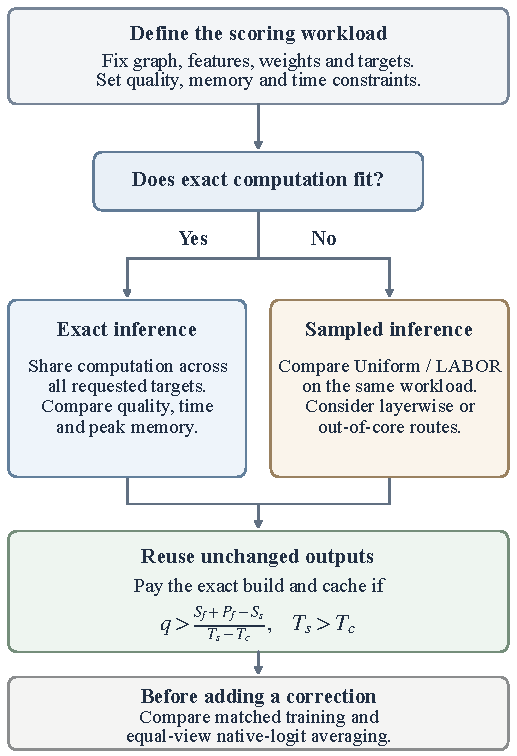
\includegraphics[width=\columnwidth]{figures/decision-guide-roman-v2/final_decision_guide.pdf}
\caption{A guide for comparing feasible prediction routes under a fixed workload and quality/memory/time constraints. Exact-output reuse requires a feasible paid build and valid cached outputs. Layerwise/out-of-core execution is a literature alternative, not evaluated here. Historical comparisons motivate matched-training and equal-view native-logit controls before a more complex correction.}
\Description{A flowchart starts from workload and quality constraints, checks output-cache validity and exact-computation feasibility, and compares feasible exact or sampled routes under measured time and memory costs.}
\label{fig:decision-guide}
\end{figure}
}
